\documentclass[11pt,a4paper]{article}

\usepackage[utf8]{inputenc} 
\usepackage[T1]{fontenc} 
\usepackage[spanish]{babel}
\decimalpoint
\setlength{\parskip}{0.5\baselineskip} 
\usepackage{fullpage}
\usepackage[procnames]{listings}
\usepackage{fancyhdr}
\usepackage{lastpage}
\usepackage{xcolor}
\usepackage{graphicx}
\usepackage[fleqn]{amsmath}
\parindent 0in 
\setlength{\mathindent}{0pt}


%% DEFINICIONES
\newcommand{\TODO}[1]{{\huge \color{red} \textbf{TODO: }#1 }}
\newcommand{\todo}[1]{{\large \color{red} \textbf{TODO: }#1 }}



\begin{document} 
\pagestyle{fancy}
\fancyhf{}
\lhead{P2: k-means (aparatado B)}
\rhead{Jesús J. Doménech Arellano, Luis Mª Costero Valero}
\rfoot{\thepage\ / \pageref{LastPage}}
\renewcommand{\headrulewidth}{0.4pt}
\renewcommand{\footrulewidth}{0.4pt}
\section*{}

\textbf{Implementar las 3 medidas de cohesión (radio, diámetro y distancia al
cuadrado promedio con respecto el centroide) para evaluar la calidad del
clustering para valores de k entre 2 y 20. Visualizar la variación de la
cohesión como un gráfico de líneas para cada una de las medidas y razonar
cuál podría ser un buen valor de k. Aparte del código, para este apartado
hay que entregar un fichero PDF incluyendo las 3 gráicas, el valor escogido
de k y su razonamiento.}


En la figuras~\ref{fig:radio},~\ref{fig:diametro}~y~\ref{fig:promedio} se
muestra la evolución de las medidas de radio, diámetro y distancia al
cuadrado promedio según se incrementa el número de clusters. La distancia
al cuadrado promedio se ha calculado teniendo en cuenta todas las
instancias con sus respectivos centroides, mientras que el radio y el
diámetro se ha realizado calculando la media aritmética entre el radio (o
diámtero) de todos los clusters. Así mismo, en estas dos últimas gráficas
se muestra la distancia máxima y mínima entre todos los clusters. 




%% A lo mejor esto sería interesante cambiarlo y ponerlo de alguna forma
%% chula, estilo 2/1, o 1/2 o 3/0 o algo así
\begin{figure}[h]
  \centering
  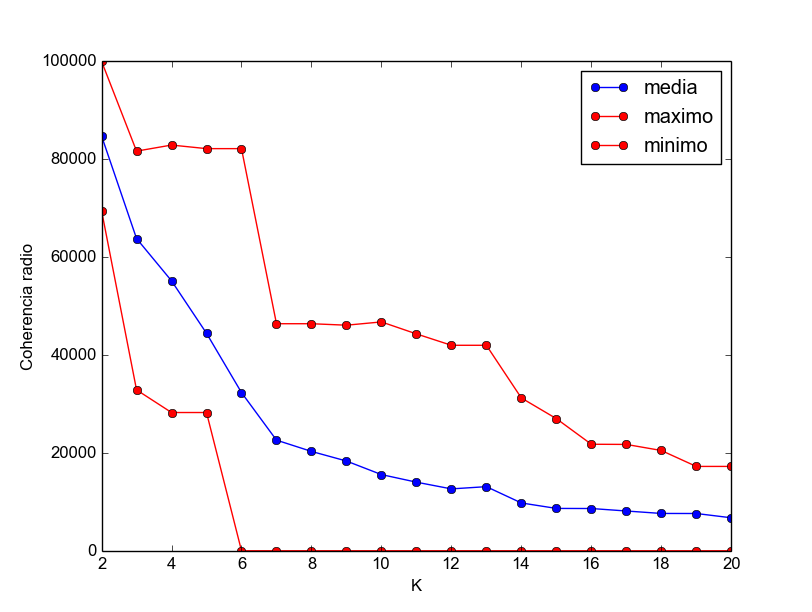
\includegraphics[width=0.6\textwidth]{img/radio_maxMin.png}
  \caption{Evolución del radio según aumenta el número de clusters}
  \label{fig:radio}
\end{figure}
\begin{figure}[h]
  \centering
  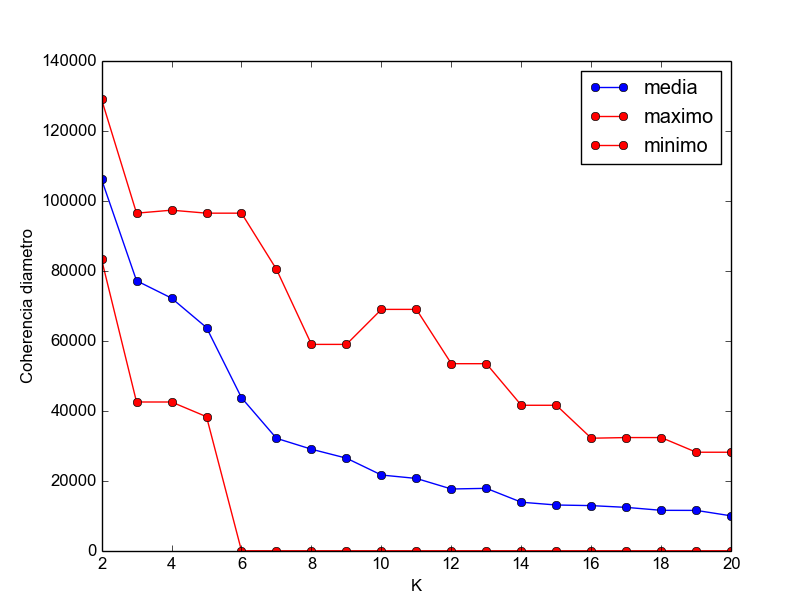
\includegraphics[width=0.6\textwidth]{img/diametro_maxMin.png}
  \caption{Evolución del diámetro según aumenta el número clusters}
  \label{fig:diametro}
\end{figure}

\begin{figure}[h]
  \centering
  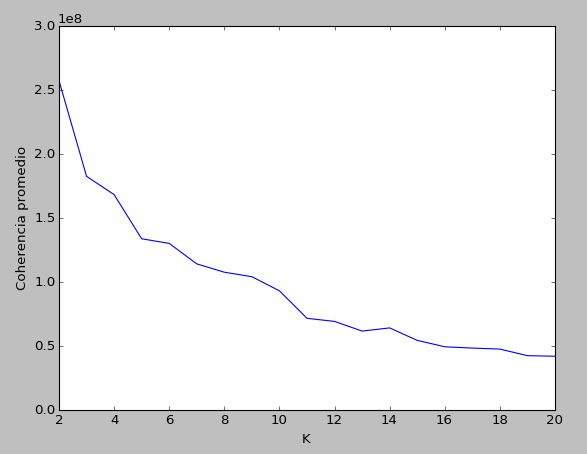
\includegraphics[width=0.6\textwidth]{img/figure_P.png}
  \caption{Evolución de la distancia al cuadrado promedio según aumenta el número
    de clusters}
  \label{fig:promedio}
\end{figure}



\hrule
\hrule

\textbf{Me estoy dando cuenta que esto no tiene mucho sentido, ya que el
  fichero tiene 440 instancias, así que este razonamiento no se si es muy
  válido o no}


Se puede observar como a partir de cierto número de clusters, la distancia
mínima es 0, ya que existen clusters donde las instancias coinciden con el
centroide o se encuentran muy próximas a él {\color{red} (¿¿??) }.



Justificar mejor: Yo creo que lo ideal es 8, ya que las distancias máximas
han bajado lo suficiente, y ya empieza a haber clusters muy pequeños. Si se
escoge un número mayor de clusters, van a ser tan pequeños que al final es
como si se trabajara con las instancias directamente, sin necesidad de agruparlas.
\end{document}
